%%%%%%%%%%%%%%%%%%%%%%%%%%%%%%%%%%%%%%%%%%%%%%%%%%%%%%%%
% Este é um documento que servirá de modelo para
% os relatórios feitos na disciplina Laboratório de Circuitos Lógicos
% 2020-2
%%%%%%%%%%%%%%%%%%%%%%%%%%%%%%%%%%%%%%%%%%%%%%%%%%%%%%%%%

%%%%%%%%%%%%%%%%%%%%%%%%%%%%%%%%%%%%%%%%%%%%%%%%%%%%%%%%%
% Use os diferentes diretórios para colocar os relatórios de cada experimento, deste modo vc consegue manter um histórico e todo material organizado em apenas um local.
% Lembre-se de mudar o Main Document no Menu!!!

\documentclass[12pt]{article}

\usepackage{sbc-template}
\usepackage[brazil,american]{babel}
\usepackage[utf8]{inputenc}

\usepackage{graphicx}
\usepackage{url}
\usepackage{float}
\usepackage{listings}
\usepackage{color}
\usepackage{todonotes}
\usepackage{algorithmic}
\usepackage{algorithm}
\usepackage{hyperref}
\usepackage{amsmath}
\usepackage{graphicx}
\usepackage{array}

\sloppy


\title{Experimento 1\\
Portas Lógicas AND, OR e NOT}

\author{Matheus Cardoso de Souza, 202033507\\
        Ualiton Ventura da Silva, 202033580\\
        Grupo G42
}

%%%% LEMBRE-SE DE MUDAR O GRUPO NA LINHA ABAIXO!!!!! %%%%%%
\address{Dep. Ciência da Computação -- Universidade de Brasília (UnB)\\
  CIC0231 - Laboratório de Circuitos Lógicos
  \email{matheus-cardoso.mc@aluno.unb.br, 202033580@aluno.unb.br}
}

\begin{document} 
\maketitle

\selectlanguage{american}
 \begin{abstract}
   This report corresponds to the Experiment 1 on ``Logical Gates \textbf{AND}, \textbf{OR} and \textbf{NOT}''.
 \end{abstract}
\selectlanguage{brazil}     
    
 \begin{resumo} 
  O presente relatório corresponde ao Experimento 1 sobre ``Portas Lógicas \textbf{AND}, \textbf{OR} e \textbf{NOT}''.
 \end{resumo}


\section{Introdução}
\label{sec:Introducao}

% Escreva com suas palavras o que vai ser trabalhado no experimento. Aqui temos um exemplo de como citar a bibliografia consultada \cite{boulic:91} \cite{smith:99}.

Neste experimento abordaremos construções de circuitos lógicos em protoboard, bem como seus respectivos funcionamentos.

\subsection{Objetivos}
\label{sec:Objetivos}

Os objetivos do presente conjunto de experimentos foram de familiarizar o aluno
com a montagem de circuitos lógicos básicos em protoboard, de permitir
mensuração de valores de tensão em diferentes pontos do circuito e também de
fonecer uma visão prática de como um determinado circuito se comporta quando
recebe diferentes valores de input.

\subsection{Materiais} 
\label{sec:Materiais}
Em função da natureza do ensino a distância, os presentes experimentos não foram
realizados usando-se materiais e equipamentos físicos, mas sim emulados por meio
da simulador online \href{https://www.tinkercad.com/}{Tinkercad}.

A seguir estão enumerados os materiais simulados:
\begin{itemize}
    \item Painel Digital
    \item \textit{Protoboard}
    \item Fios
    \item Seletores de estado lógico
    \item LEDs
    \item Resistores
    \item Multímetros
    \item Portas Lógicas \textbf{AND}, \textbf{OR} e \textbf{NOT}
\end{itemize}

\section{Procedimentos}
\label{sec:Procedimentos}

Passaremos a apresentar os experimentos requeridos.

\subsection{LED ligado a uma chave, e sua tensão}
\label{sec:led_chave}

Nesse experimento o objetivo era que ligássemos um LED a uma chave, e depois
verificássemos se ele acende e apaga corretamente quando a chave é acionada.
Também deveríamos medir o valor da tensão de alimentação com um multímetro o
valor da tensão de alimentação.\\
Para conferir o vídeo deste experimento, acessse o seguinte link:
\href{https://youtu.be/raLr9IothuI}{https://youtu.be/raLr9IothuI}.

\begin{figure}[H]
    \centering
    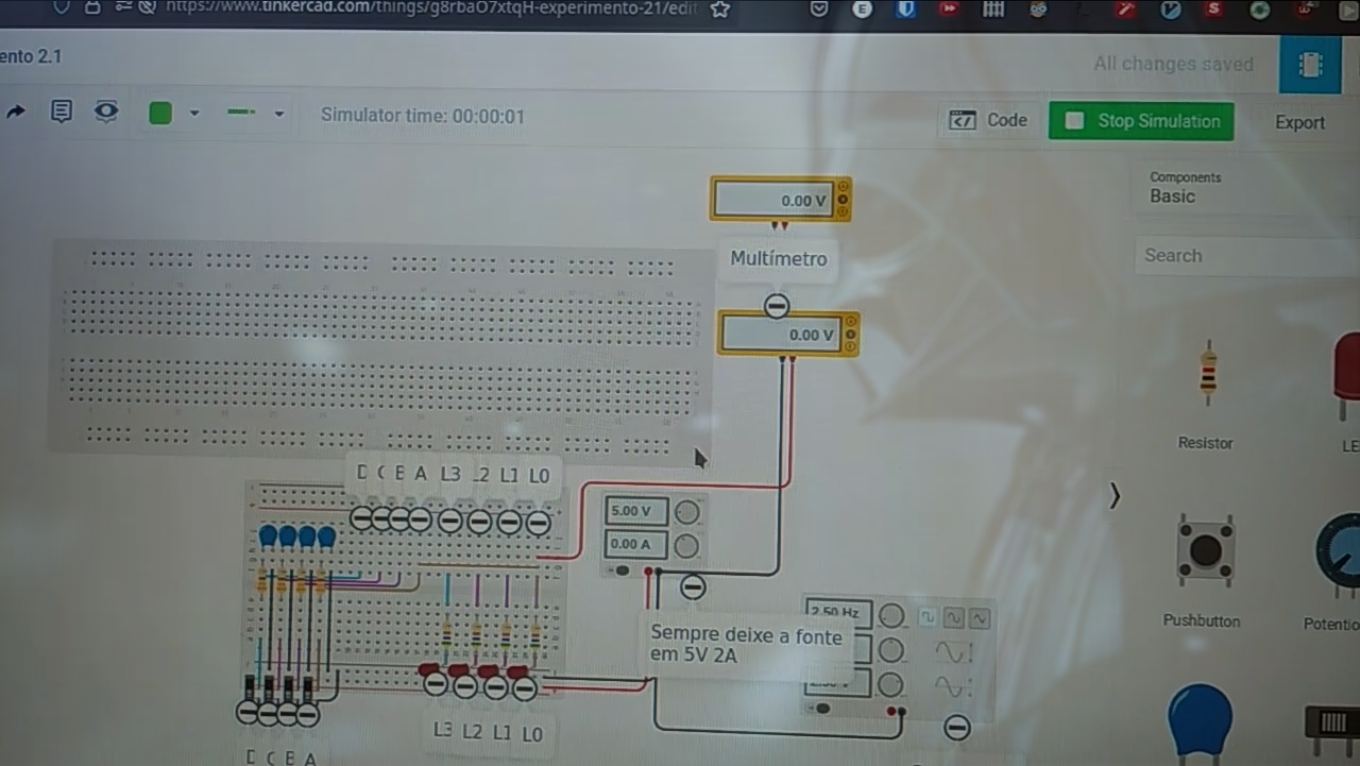
\includegraphics[width=.9\textwidth]{exp1_2.1_f1.png}
    \caption{Chave aberta, LED desligado.}
    \label{fig:exp1_2.1_f1}
\end{figure}

\begin{figure}[H]
    \centering
    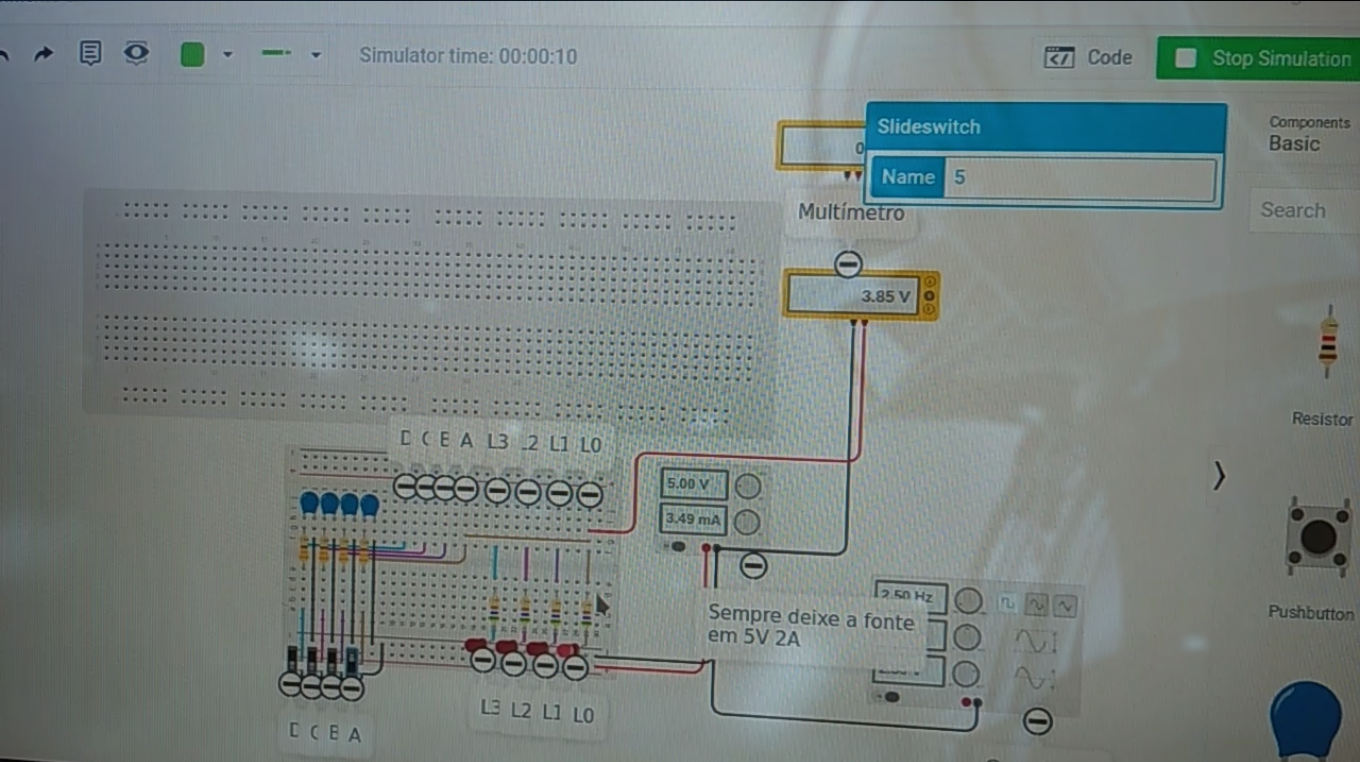
\includegraphics[width=.9\textwidth]{exp1_2.1_f2.png}
    \caption{Chave fechada, LED ligado.}
    \label{fig:exp1_2.1_f2}
\end{figure}

Como podemos notar com a figura \ref{fig:exp1_2.1_f1}, quando a chave \textbf{A}
está desligada temos que o LED \textbf{L0} está apagado, e também podemos ver
que o multímetro afere uma voltagem de \( 0.00V \). Agora, quando acionamos a
chave \textbf{A}, o LED \textbf{L0} acende, e a tensão de alimentação é de
\( 3.85V \). Logo, podemos concluir que o valor pedido no enunciado deste
experimento é \( VCC = 3.85V \).
\\[2em]

\subsection{Diferença entre portas lógicas \textbf{AND} e \textbf{OR}}
\label{sec:and_e_or}

Este experimento tinha como objetivo verificarmos a diferença de comportamento
entre circuitos criados com portas lógicas \textbf{AND} e \textbf{OR}.\\
Para conferir o vídeo deste experimento, acesse o seguinte link:
\href{https://youtu.be/DRLLBkMOeeA}{https://youtu.be/DRLLBkMOeeA}.

\begin{table}[H]
    \centering
    \caption{Tabela para a porta lógica \textbf{AND}}
    \begin{tabular}{|c|c|c|c|c|c|}
    \hline
    \textbf{B} & \textbf{A} & \textbf{L3}=S4 & \textbf{L2}=S3 & \textbf{L1}=S2 & \textbf{L0}=S1 \\
    \hline
    0  & 0 & \(0 = 0V\) & \(0 = 0V\) & \(0 = 0V\) & \(0 = 0V\) \\
    \hline
    0  & 1 & \(0 = 0V\) & \(0 = 0V\) & \(0 = 0V\) & \(0 = 0V\) \\
    \hline
    1  & 0 & \(0 = 0V\) & \(0 = 0V\) & \(0 = 0V\) & \(0 = 0V\) \\
    \hline
    1  & 1 & \(1 = 4.77V\) & \(1 = 4.77V\) & \(1 = 4.77V\) & \(1 = 4.77V\) \\
    \hline
    \end{tabular}
    \label{tab:tabela_and}
\end{table}

\begin{table}[H]
    \centering
    \caption{Tabela para a porta lógica \textbf{OR}}
    \begin{tabular}{|c|c|c|c|c|c|}
    \hline
    \textbf{B} & \textbf{A} & \textbf{L3}=S4 & \textbf{L2}=S3 & \textbf{L1}=S2 & \textbf{L0}=S1 \\
    \hline
    0  & 0 & \(0 = 0V\) & \(0 = 0V\) & \(0 = 0V\) & \(0 = 0V\) \\
    \hline
    0  & 1 & \(1 = 4.77V\) & \(1 = 4.77V\) & \(1 = 4.77V\) & \(1 = 4.77V\) \\
    \hline
    1  & 0 & \(1 = 4.77V\) & \(1 = 4.77V\) & \(1 = 4.77V\) & \(1 = 4.77V\) \\
    \hline
    1  & 1 & \(1 = 4.77V\) & \(1 = 4.77V\) & \(1 = 4.77V\) & \(1 = 4.77V\) \\
    \hline
    \end{tabular}
    \label{tab:tabela_or}
\end{table}

Como podemos notar pelo vídeo e também com o resultado da tabela, o
funcionamento das portas lógicas \textbf{AND} e \textbf{OR} é como o esperado.
\\[2em]

\subsection{Porta lógica \textbf{AND} apenas com portas \textbf{OR} e \textbf{NOT}}
\label{sec:and_with_only_or_and_not}

Nesse experimento, o objetivo foi planejarmos e implementarmos uma porta lógica
\textbf{AND} usando apenas portas \textbf{OR} e \textbf{NOT}.\\
Para conferir o vídeo deste experimento, acesse o seguinte link:
\href{https://youtu.be/PZo3VhjNYEg}{https://youtu.be/PZo3VhjNYEg}.

\begin{figure}[H]
    \centering
    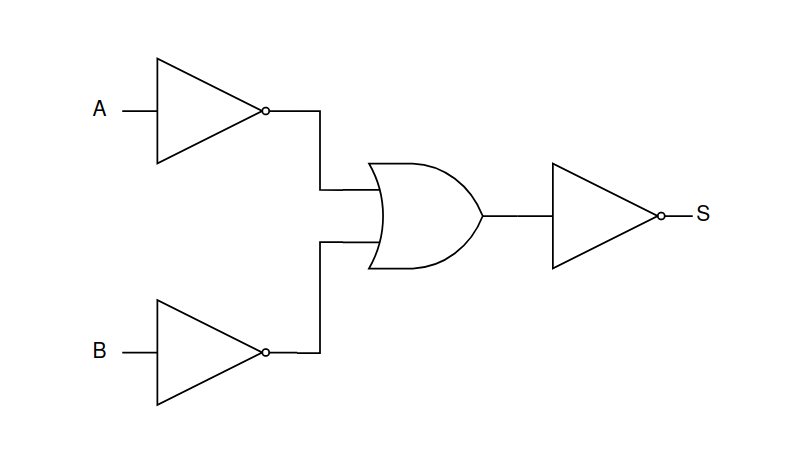
\includegraphics[width=.9\textwidth]{exp1_2.3_f1.png}
    \caption{Esquema de uma porta \textbf{AND} apenas com portas \textbf{OR} e \textbf{NOT}}
    \label{fig:exp1_2.3_f1}
\end{figure}

Temos que a figura \ref{fig:exp1_2.3_f1} representa corretamente a emulação de
uma porta \textbf{AND}, mesmo sendo construida apenas com portas \textbf{OR} e
\textbf{NOT}. Esse comportamento pode ser explicado pela seguinte equação
lógica:

\begin{align}
\lnot (\lnot A \lor \lnot B) &\equiv \\
\lnot (\lnot A) \land \lnot (\lnot B) &\equiv \\
A \land B \label{eq:and1}
\end{align}

Dessa forma, pela equação \ref{eq:and1}, temos que nosso esquema representado na figura
\ref{fig:exp1_2.3_f1} é equivalente a uma porta lógica \textbf{AND}.

\begin{table}[H]
    \centering
    \caption{Tabela para a porta lógica \textbf{AND}}
    \begin{tabular}{|c|c|c|c|}
    \hline
    \textbf{B} & \textbf{A} & \textbf{L0}=A.B & \textbf{Esquema} \\
    \hline
    0 & 0 & 0 & \multirow{}{}{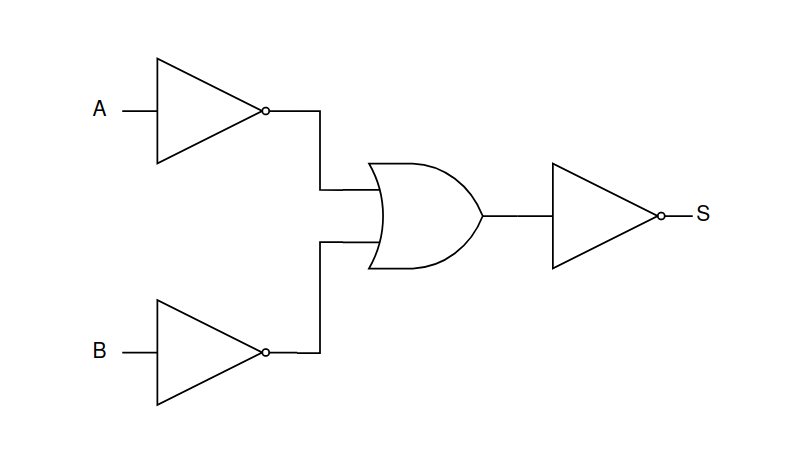
\includegraphics[width=.7\textwidth]{exp1_2.3_f1.png}} \\ \cline{1-3}
    0 & 1 & 0 &  \\ \cline{1-3}
    1 & 0 & 0 &  \\ \cline{1-3}
    1 & 1 & 1 &  \\ \hline
    \end{tabular}
    \label{tab:tabela_and}
\end{table}

Foi-nos requerido que preenchêssemos uma tabela contendo todos os estados
lógicos da combinação de valores para \textbf{A} e \textbf{B}. A tabela
\ref{tab:tabela_and} nos fornece todos os valores possíveis para tais
combinações.

\section{Análise dos Resultados}
\label{sec:Resultados}

Como pudemos notar com os experimentos realizados, é possível criarmos circuitos
lógicos que seguem a lógica booleana, realizando operações de \textbf{AND},
\textbf{NOT} e \textbf{OR} usando circuitos elétricos.

\section{Conclusão}
\label{sec:Conclusao}

Pudemos observar o comportamento correto e esperado dos circuitos lógicos
montados. Entretanto, devido ao fato de utilizarmos uma ferramenta de simulação,
não pudemos observar os fenômenos esperados de leves variações de voltagem no
circuito elétrico, pois todo o circuito é considerado ideal no Tinkercad.

\nocite{*}
\bibliographystyle{sbc}
\bibliography{relatorio}  %Aqui é a definição do arquivo .bib a ser usado pelas referências


\newpage 
% Colocar aqui apenas as respostas dos itens da Auto-Avaliação
\section*{Auto-Avaliação}

\subsection{Com relação aos níveis lógicos TTL de entrada e saída, assinale a
  alternativa correta}
Resposta: Item \textbf{B}.

\subsection{Assinale os conjuntos universais dentre os conjuntos abaixo}
Resposta: Item \textbf{A}.

\subsection{Preencha a tabela verdade do circuito abaixo}
\begin{figure}[H]
    \centering
    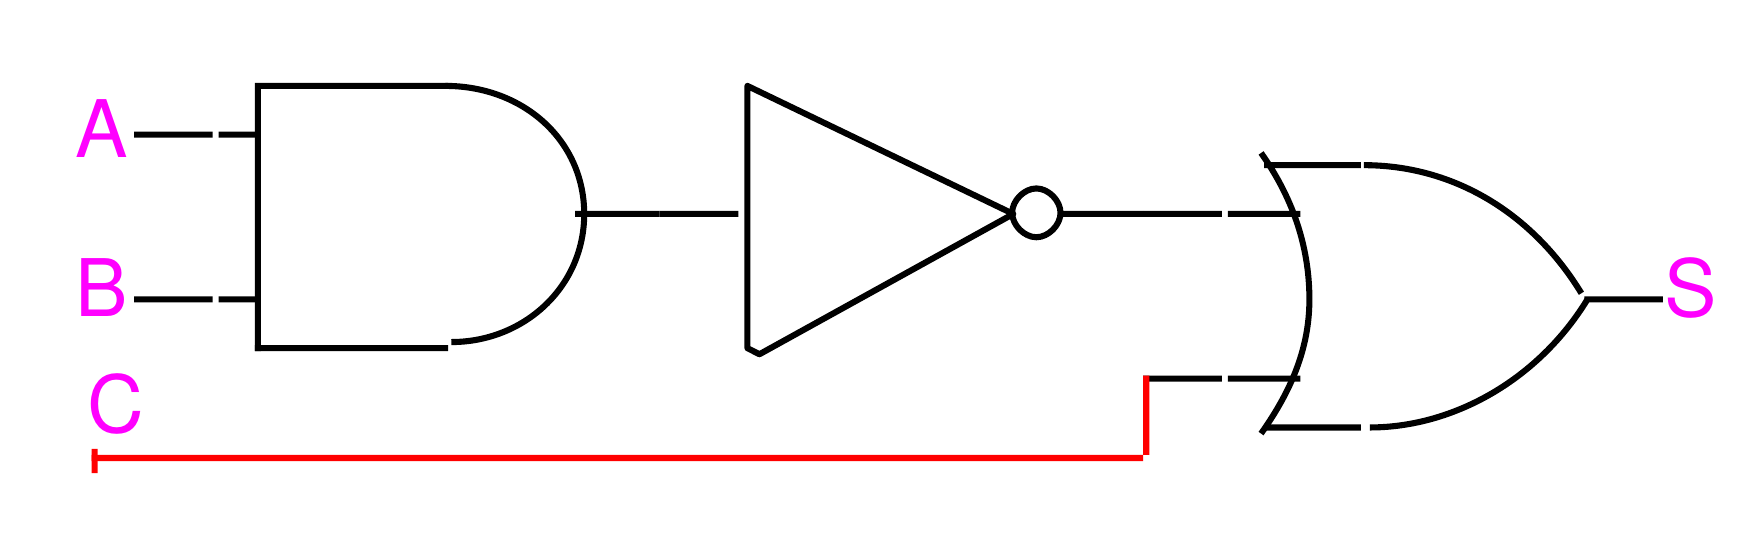
\includegraphics[width=.9\textwidth]{exp1_4.3_f1.png}
    \caption{Circuito da questão}
    \label{fig:exp1_4.3_f1}
\end{figure}

Resposta:

\begin{table}[H]
    \centering
    \caption{Tabela com a resposta para a questão}
    \begin{tabular}{|c|c|c|c|} \hline
    \textbf{A} & \textbf{B} & \textbf{C} & \textbf{S} \\ \hline
    0 & 0 & 0 & 1 \\ \hline
    0 & 0 & 1 & 1 \\ \hline
    0 & 1 & 0 & 1 \\ \hline
    0 & 1 & 1 & 1 \\ \hline
    1 & 0 & 0 & 1 \\ \hline
    1 & 0 & 1 & 1 \\ \hline
    1 & 1 & 0 & 0 \\ \hline
    1 & 1 & 1 & 1 \\ \hline
    \end{tabular}
    \label{tab:tabela_verdade}
\end{table}


\end{document}
